
\chapter{Vectorizations' Stability Theorems} \label{chap:vectorizations}

The study of stability in topological data analysis is crucial for ensuring that small perturbations in the input data lead to controlled changes in its topological representations. This chapter explores various vectorization methods—persistence landscapes, persistence images, and Euler curves—and their associated stability theorems. By establishing bounds on how these vectorizations change with respect to distances between persistence modules or diagrams, we gain a deeper understanding of their robustness in practical applications.

Section \ref{sec:landscapes} reviews the results of the 2015 paper from Peter Bubenik \cite{bubenik}. Section \ref{sec:images} follows the 2020 paper Henry Adams et al. \cite{adams} and Section \ref{sec:euler-curves} presents the results from Paweł Dłotko and Davide Gurnari 2023 paper, \cite{dlotko}.

\section{Persistence landscapes} \label{sec:landscapes}

Persistence landscapes provide a functional summary of persistence diagrams, converting them into a sequence of real-valued functions that capture topological features in a more tractable form. This section introduces the definition of persistence landscapes, their key properties, and stability results that relate the landscape distance to the bottleneck and Wasserstein distances between persistence diagrams.

Recall from Definition \ref{def:persistent-homology} that given some persistence module $ (V, \pi) $ and a fixed $k$ the $k$-th persistent Betti number associated to $ x \leq y \in \R $ is given by
\begin{equation}
    \beta_x^y(V) = \dim (\im \pi_{x \leq y}).
\end{equation}

\begin{lemma}[Lemma 1, \cite{bubenik}] \label{lemma:landscapes-aux-1}
    Let $ (V, \pi) $ be a persistence module and let $ a \leq b \leq c \leq d \in \R $. Then $ \beta_b^c \geq \beta_a^d $.
\end{lemma}
\begin{proof}
    Since $ \pi_{a \leq d} = \pi_{c \leq d} \circ \pi_{b \leq c} \circ \pi_{a \leq b} $, the dimension of the image of $ \pi_{a \leq d} $ must be smaller than the one of just $ \pi_{b \leq c} $.
\end{proof}

\begin{definition}[Rank function]
    The {\bf rank function} of a persistence module $ V $ is the function $ \delta \colon \R^2 \to \R $ given by
    \begin{equation}
        \lambda(b, d) = \begin{cases}
            \beta_b^d &\text{ if }  b \leq d \\
            0 &\text{ otherwise}.
        \end{cases}
    \end{equation}
    We can change coords to define an analogous function but defined on the upper half plane. Let
    \begin{align}
        &m = \frac{b + d}{2}, & &h = \frac{d-b}{2}.
    \end{align}
    The {\bf rescaled rank function} is the function $ \delta \colon \R^2 \to \R $ given by
    \begin{equation}
        \lambda(m, h) = \begin{cases}
        \beta^{m-h, m+h} &\text{ if } \geq 0,\\
        0 & \text{ otherwise}.
        \end{cases}
    \end{equation}
\end{definition}

\begin{lemma}[Lemma 2, \cite{bubenik}] \label{lemma:landscapes-aux-2}
    Let $ 0 \leq h_1 \leq h_2 $ be real numbers. Then $ \beta_{t-h_1}^{t+h_1} \geq \beta_{t-h_2}^{t+h_2} $.
\end{lemma}
\begin{proof}
    As $ t - h_2 \leq t-h_1 \leq t+h_1 \leq t+h_2$, the inequality comes from Lemma \ref{lemma:landscapes-aux-1}.
\end{proof}

Let $ \overline{\R} \coloneq \R \cup \{-\infty, \infty\} $ denote the extended real numbers. 

\begin{definition}[Persistence landscape] \label{def:persistence-landscape}
    A {\bf persistence landscape} is a function $ \lambda \colon \N \times \R \to \overline \R $, defined as
    \begin{equation}
        \lambda(k, t) \coloneq \sup \{ m \geq 0 \mid \beta^{t-m, t+m} \geq k\}.
    \end{equation}
    Note that this function can also be seen as a sequence of function $ \lambda_k \colon \R \to \overline{\R} $, where $ \lambda_k(t) = \lambda(k, t) $.
\end{definition}

\begin{definition}[$K$-Lipschitz]
    Let $ (X, d_X) $, $ (Y, d_Y) $ be two metric spaces and let $ K > 0 $. A {\bf $K$-Lipschitz} map is a map $ f \colon (X, d_X) \to (Y, d_Y) $, such that for every $ x_1, x_2 \in X $, 
    \begin{equation}
        d_Y(f(x_1), f(x_2)) \leq K d_X(x_1, x_2).
    \end{equation}
\end{definition}

\begin{lemma}[Lemma 3, \cite{bubenik}] \label{lemma:landscapes-aux-3}
    Let $ \lambda_k \colon \R \to \overline{\R} $ be an element of a persistence landscape. The following properties are verified.
    \begin{enumerate}
        \item $\lambda_k(t) \geq 0$,
        \item $\lambda_k(t) \geq \lambda_{k+1}(t)$,
        \item $\lambda_k$ is $1$-Lipschitz, that is, for $ t, s \in \R $, $ | \lambda_k(t) - \lambda_k(s) | \leq |t-s| $.
    \end{enumerate}
\end{lemma}
\begin{proof}
    Properties 1. and 2. came directly from the definition. For 3., suppose $ \lambda_k(s) \leq \lambda_k(t) $. If $ \lambda_k(t) \leq |t -s | $ then, of course, $ \lambda_k(t) - \lambda_k(s) \leq \lambda_k(t) \leq |t-s| $. Else, if $ \lambda_k(t) >  |t - s | $, we can take some $ h \in (0, \lambda_k(t) -  |t - s |) $ verifying
    \begin{equation}
        t - \lambda_k(t) < s- h < s + h < t + \lambda_k(t).
    \end{equation}
    Hence, by Lemma \ref{lemma:landscapes-aux-1} we have $ \beta_{s-h}^{s+h} \geq k $ and $ \lambda_k(s) \geq \lambda_k(t) - |t -s| $. Therefore, $ \lambda_k(t) - \lambda_k(s) \leq |t-s| $.
\end{proof}

\begin{example}[Persistence landscape]
    Figure \ref{fig:persistance-landscapes} shows the rank function, the rescaled rank function and the persistence diagram of one of the persistence diagrams of Example \ref{ex:wasserstein}.
    \begin{figure}[H] 
        \centering
        \begin{subfigure}[b]{0.45\linewidth}
            \centering
            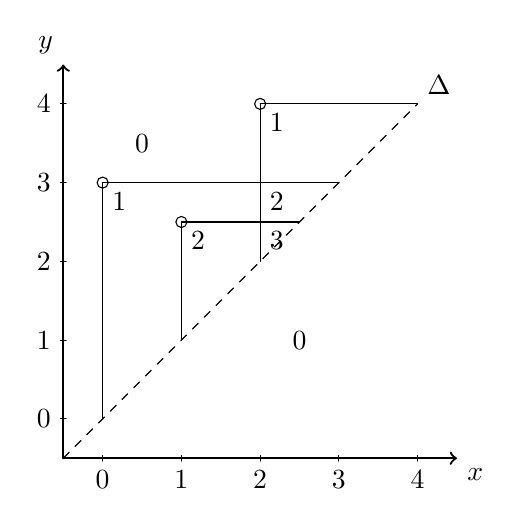
\begin{tikzpicture}[line cap=round, line join=round, x=1cm, y=1cm]
                
                \draw[thick,->] (0,0) -- (5,0) node[anchor=north west] {$x$};
                \draw[thick,->] (0,0) -- (0,5) node[anchor=south east] {$y$};
                \draw[dashed] (0,0) -- (4.5,4.5) node[above right] {$\Delta$};

                \draw (0.5 cm,1pt) -- (0.5 cm,-1pt) node[anchor=north] {0};
                \draw (1.5 cm,1pt) -- (1.5 cm,-1pt) node[anchor=north] {1};
                \draw (2.5 cm,1pt) -- (2.5 cm,-1pt) node[anchor=north] {2};
                \draw (3.5 cm,1pt) -- (3.5 cm,-1pt) node[anchor=north] {3};
                \draw (4.5 cm,1pt) -- (4.5 cm,-1pt) node[anchor=north] {4};

                \draw (1pt,0.5 cm) -- (-1pt,0.5 cm) node[anchor=east] {0};
                \draw (1pt,1.5 cm) -- (-1pt,1.5 cm) node[anchor=east] {1};
                \draw (1pt,2.5 cm) -- (-1pt,2.5 cm) node[anchor=east] {2};
                \draw (1pt,3.5 cm) -- (-1pt,3.5 cm) node[anchor=east] {3};
                \draw (1pt,4.5 cm) -- (-1pt,4.5 cm) node[anchor=east] {4};

                \draw (1.5, 3) circle (2pt) node[below right] {2};
                \draw (0.5, 3.5) circle (2pt) node[below right] {1};
                \draw (2.5, 4.5) circle (2pt) node[below right] {1};

                \draw (3, 1.5) node {0};
                \draw (1, 4) node {0};
                \draw (2.5, 3.5) node[below right] {2};
                \draw (2.5, 3) node[below right] {3};

                \draw (1.5, 3) -- (1.5, 1.5);
                \draw (1.5, 3) -- (3, 3);
                \draw (0.5, 3.5) -- (0.5, 0.5);
                \draw (0.5, 3.5) -- (3.5, 3.5);
                \draw (2.5, 4.5) -- (2.5, 2.5);
                \draw (2.5, 4.5) -- (4.5, 4.5);
                
            \end{tikzpicture}
            \caption{Rank function.}
        \end{subfigure}
        \hfill
        \begin{subfigure}[b]{0.45\linewidth}
            \centering
            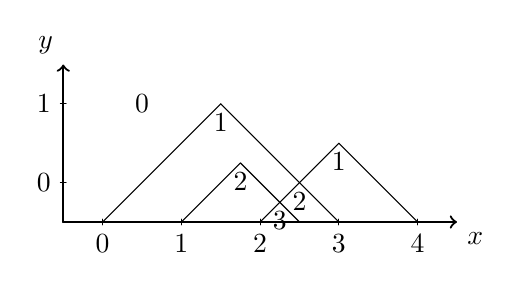
\begin{tikzpicture}[line cap=round, line join=round, x=1cm, y=1cm]
                
                \draw[thick,->] (0,0) -- (5,0) node[anchor=north west] {$x$};
                \draw[thick,->] (0,0) -- (0,2) node[anchor=south east] {$y$};

                \draw (0.5 cm,1pt) -- (0.5 cm,-1pt) node[anchor=north] {0};
                \draw (1.5 cm,1pt) -- (1.5 cm,-1pt) node[anchor=north] {1};
                \draw (2.5 cm,1pt) -- (2.5 cm,-1pt) node[anchor=north] {2};
                \draw (3.5 cm,1pt) -- (3.5 cm,-1pt) node[anchor=north] {3};
                \draw (4.5 cm,1pt) -- (4.5 cm,-1pt) node[anchor=north] {4};

                \draw (1pt,0.5 cm) -- (-1pt,0.5 cm) node[anchor=east] {0};
                \draw (1pt,1.5 cm) -- (-1pt,1.5 cm) node[anchor=east] {1};

                \draw (2.25, 0.75) node[below] {2};
                \draw (2.0, 1.5) node[below] {1};
                \draw (3.5, 1.0) node[below] {1};

                \draw (1, 1.5) node {0};
                \draw (3, 0.5) node[below] {2};
                \draw (2.75, 0.25) node[below] {3};

                \draw (2.25, 0.75) -- (1.5, 0);
                \draw (2.25, 0.75) -- (3.0, 0);
                \draw (2.0, 1.5) -- (0.5, 0);
                \draw (2.0, 1.5) -- (3.5, 0);
                \draw (3.5, 1.0) -- (2.5, 0);
                \draw (3.5, 1.0) -- (4.5, 0);
                
            \end{tikzpicture}
            \caption{Rescaled rank function.}
        \end{subfigure}
        \begin{subfigure}[b]{\linewidth}
            \centering
            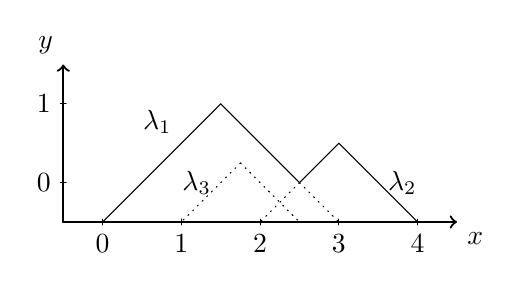
\begin{tikzpicture}[line cap=round, line join=round, x=1cm, y=1cm]
                
                \draw[thick,->] (0,0) -- (5,0) node[anchor=north west] {$x$};
                \draw[thick,->] (0,0) -- (0,2) node[anchor=south east] {$y$};

                \draw (0.5 cm,1pt) -- (0.5 cm,-1pt) node[anchor=north] {0};
                \draw (1.5 cm,1pt) -- (1.5 cm,-1pt) node[anchor=north] {1};
                \draw (2.5 cm,1pt) -- (2.5 cm,-1pt) node[anchor=north] {2};
                \draw (3.5 cm,1pt) -- (3.5 cm,-1pt) node[anchor=north] {3};
                \draw (4.5 cm,1pt) -- (4.5 cm,-1pt) node[anchor=north] {4};

                \draw (1pt,0.5 cm) -- (-1pt,0.5 cm) node[anchor=east] {0};
                \draw (1pt,1.5 cm) -- (-1pt,1.5 cm) node[anchor=east] {1};

                \draw[dotted] (2.25, 0.75) -- (1.5, 0);
                \draw[dotted] (2.25, 0.75) -- (3.0, 0);
                \draw (2.0, 1.5) -- (0.5, 0);
                \draw (2.0, 1.5) -- (3, 0.5);
                \draw[dotted] (3, 0.5) -- (3.5, 0);
                \draw (3.5, 1.0) -- (3, 0.5);
                \draw[dotted] (3, 0.5) -- (2.5, 0);
                \draw (3.5, 1.0) -- (4.5, 0);

                \draw (1.5, 1) node[above left] {$\lambda_1$};
                \draw (2, 0.5) node[left] {$\lambda_3$};
                \draw (4, 0.5) node[right] {$\lambda_2$};
                
            \end{tikzpicture}
            \caption{Persistence landscape.}
        \end{subfigure}
        \caption{Persistence landscape of a persistence diagram.}
        \label{fig:persistance-landscapes}
    \end{figure}
\end{example}

\begin{example}
    One of the main advantages of persistence landscapes in comparison with persistence diagrams is that they count with a nice geometry to work with. For example, in Figure \ref{fig:landscape-means} we can see how meanwhile persistence diagrams might not have a unique mean, persistence landscapes do have.
    \begin{figure}[H]
        \begin{figure}[H] 
    \centering
    \begin{subfigure}[b]{0.45\linewidth}
        \centering
        \begin{tikzpicture}[line cap=round, line join=round, x=1cm, y=1cm]
            
            \draw[thick,->] (0,0) -- (4,0) node[anchor=north west] {$x$};
            \draw[thick,->] (0,0) -- (0,4) node[anchor=south east] {$y$};

            \draw (0 cm,1pt) -- (0 cm,-1pt) node[anchor=north] {0};
            \draw (1 cm,1pt) -- (1 cm,-1pt) node[anchor=north] {1};
            \draw (2 cm,1pt) -- (2 cm,-1pt) node[anchor=north] {2};
            \draw (3 cm,1pt) -- (3 cm,-1pt) node[anchor=north] {3};

            \draw (1pt,0 cm) -- (-1pt,0 cm) node[anchor=east] {0};
            \draw (1pt,1 cm) -- (-1pt,1 cm) node[anchor=east] {1};
            \draw (1pt,2 cm) -- (-1pt,2 cm) node[anchor=east] {2};
            \draw (1pt,3 cm) -- (-1pt,3 cm) node[anchor=east] {3};

            \draw (1, 2) circle (2pt);
            \draw (3, 2) circle (2pt);

            \draw[fill=black] (2, 1) circle (2pt);
            \draw[fill=black] (2, 3) circle (2pt);

            \draw (1.5, 2.5) node {$\cdot$};
            \draw (2.5, 1.5) node {$\cdot$};

            \draw (1.5, 1.5) node {$\ast$};
            \draw (2.5, 2.5) node {$\ast$};
            
        \end{tikzpicture}
        \caption{}
        \label{fig:means-a}
    \end{subfigure}
    \begin{subfigure}[b]{0.45\linewidth}
        \centering
        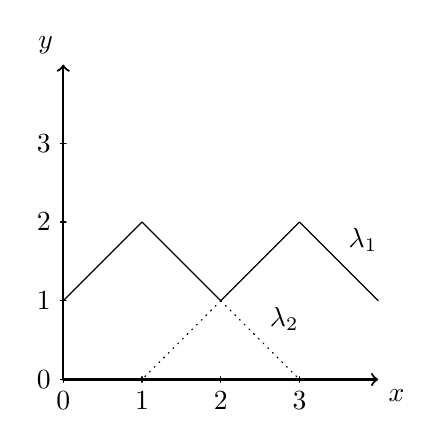
\begin{tikzpicture}[line cap=round, line join=round, x=1cm, y=1cm]
            
            \draw[thick,->] (0,0) -- (4,0) node[anchor=north west] {$x$};
            \draw[thick,->] (0,0) -- (0,4) node[anchor=south east] {$y$};

            \draw (0 cm,1pt) -- (0 cm,-1pt) node[anchor=north] {0};
            \draw (1 cm,1pt) -- (1 cm,-1pt) node[anchor=north] {1};
            \draw (2 cm,1pt) -- (2 cm,-1pt) node[anchor=north] {2};
            \draw (3 cm,1pt) -- (3 cm,-1pt) node[anchor=north] {3};

            \draw (1pt,0 cm) -- (-1pt,0 cm) node[anchor=east] {0};
            \draw (1pt,1 cm) -- (-1pt,1 cm) node[anchor=east] {1};
            \draw (1pt,2 cm) -- (-1pt,2 cm) node[anchor=east] {2};
            \draw (1pt,3 cm) -- (-1pt,3 cm) node[anchor=east] {3};

            \draw (0, 1) -- (1, 2) -- (2, 1);
            \draw[dotted] (2, 1) -- (3,0);

            \draw (2, 1) -- (3, 2) -- (4, 1);
            \draw[dotted] (2, 1) -- (1,0);

            \draw (2.5, 0.5) node[above right] {$\lambda_2$};
            \draw (3.5, 1.5) node[above right] {$\lambda_1$};
            
        \end{tikzpicture}
        \caption{}
        \label{fig:means-b}
    \end{subfigure}
    \begin{subfigure}[b]{0.45\linewidth}
        \centering
        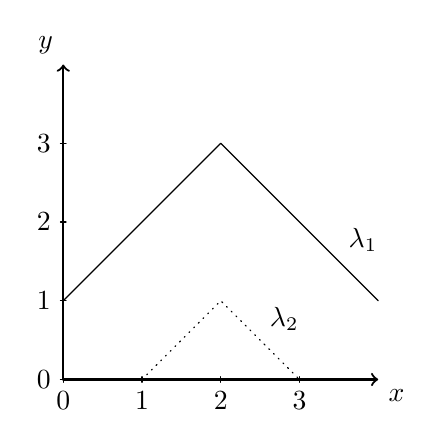
\begin{tikzpicture}[line cap=round, line join=round, x=1cm, y=1cm]
            
            \draw[thick,->] (0,0) -- (4,0) node[anchor=north west] {$x$};
            \draw[thick,->] (0,0) -- (0,4) node[anchor=south east] {$y$};

            \draw (0 cm,1pt) -- (0 cm,-1pt) node[anchor=north] {0};
            \draw (1 cm,1pt) -- (1 cm,-1pt) node[anchor=north] {1};
            \draw (2 cm,1pt) -- (2 cm,-1pt) node[anchor=north] {2};
            \draw (3 cm,1pt) -- (3 cm,-1pt) node[anchor=north] {3};

            \draw (1pt,0 cm) -- (-1pt,0 cm) node[anchor=east] {0};
            \draw (1pt,1 cm) -- (-1pt,1 cm) node[anchor=east] {1};
            \draw (1pt,2 cm) -- (-1pt,2 cm) node[anchor=east] {2};
            \draw (1pt,3 cm) -- (-1pt,3 cm) node[anchor=east] {3};

            \draw (0, 1) -- (2, 3) -- (4, 1);
            \draw[dotted] (1,0) -- (2, 1) -- (3,0);

            \draw (2.5, 0.5) node[above right] {$\lambda_2$};
            \draw (3.5, 1.5) node[above right] {$\lambda_1$};
            
        \end{tikzpicture}
        \caption{}
        \label{fig:means-c}
    \end{subfigure}
    \begin{subfigure}[b]{0.45\linewidth}
        \centering
        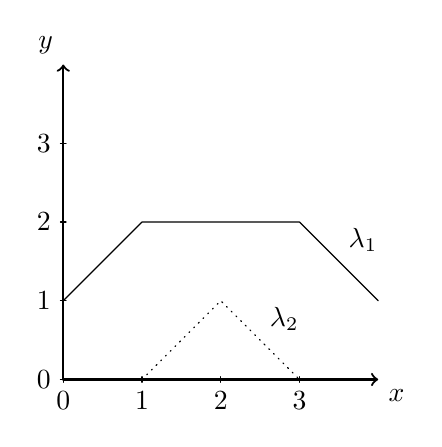
\begin{tikzpicture}[line cap=round, line join=round, x=1cm, y=1cm]
            
            \draw[thick,->] (0,0) -- (4,0) node[anchor=north west] {$x$};
            \draw[thick,->] (0,0) -- (0,4) node[anchor=south east] {$y$};

            \draw (0 cm,1pt) -- (0 cm,-1pt) node[anchor=north] {0};
            \draw (1 cm,1pt) -- (1 cm,-1pt) node[anchor=north] {1};
            \draw (2 cm,1pt) -- (2 cm,-1pt) node[anchor=north] {2};
            \draw (3 cm,1pt) -- (3 cm,-1pt) node[anchor=north] {3};

            \draw (1pt,0 cm) -- (-1pt,0 cm) node[anchor=east] {0};
            \draw (1pt,1 cm) -- (-1pt,1 cm) node[anchor=east] {1};
            \draw (1pt,2 cm) -- (-1pt,2 cm) node[anchor=east] {2};
            \draw (1pt,3 cm) -- (-1pt,3 cm) node[anchor=east] {3};

            \draw (0, 1) -- (1,2) -- (3,2) -- (4, 1);
            \draw[dotted] (1,0) -- (2, 1) -- (3,0);

            \draw (2.5, 0.5) node[above right] {$\lambda_2$};
            \draw (3.5, 1.5) node[above right] {$\lambda_1$};
            
        \end{tikzpicture}
        \caption{}
        \label{fig:means-d}
    \end{subfigure}
    \caption[Means from persistence landscapes]{The rescaled persistence diagrams of \ref{fig:means-a}, $\{(1, 2), (3, 2)\}$ and $\{(2, 1), (2, 3)\}$ have two (Fréchet) means: $\{(1.5, 2.5), (2.5, 1.5)\}$ and $\{(1.5, 1.5), (2.5, 2.5)\}$. In contrast, their corresponding persistence landscapes \ref{fig:means-b} and \ref{fig:means-c} have a unique mean \ref{fig:means-d}.}
    \label{fig:landscape-means}
\end{figure}
    \end{figure}
\end{example}

\begin{definition}[$p$-landscape distance]
    Let $ W $ and $ W $ be two persistence modules, and let $ \lambda $ and $ \lambda' $ its corresponding persistence landscapes. Let $ 1 \leq p \leq \infty $. The {\bf $p$-landscape distance between persistence modules} $ V $ and $ W $ is defined as
    \begin{equation}
        \Lambda_p(V, W) \coloneq \|\lambda - \lambda' \|_p.
    \end{equation}
    Similarly, if $ D $ and $ D' $ are two persistence diagrams, and are $ \lambda $ and $ \lambda' $ its corresponding persistence landscapes, The {\bf $p$-landscape distance between persistence diagrams} $ V $ and $ W $ is defined as
    \begin{equation}
        \Lambda_p(D, D') \coloneq \|\lambda - \lambda' \|_p.
    \end{equation}
\end{definition}

\begin{theorem}[Theorem 17, \cite{bubenik}] \label{theorem:landscapes-aux}
    Let $ (V, \pi) $ and $ (W, \theta) $ two persistence modules. Then their $\infty$-landscape distance between them is a lower bound of their interleaving distance. That is
    \begin{equation}
        \Lambda_{\infty}(V, W) \leq \di(V, W)
    \end{equation}
\end{theorem}
\begin{proof}
    Suppose $ V $ and $ W $ are $\delta$-interleaved, recall definition \ref{def:interleaved-modules}. Then, considering $ \pi_{t-m \leq t+m} $ and $ \pi_{t-m + \delta \leq t+m - \delta } $, we have that $ t-m \leq t-m + \delta \leq t+m - \delta \leq t+m $, hence by Lemma \ref{lemma:landscapes-aux-1} we have
    \begin{equation}
        \beta_{t-m+\delta}^{t+m-\delta}(W) \geq \beta_{t-m}^{t+m}(V).
    \end{equation}
    Now if $ \delta $ and $ \delta' $ are the corresponding persistence landscapes of $ V $ and $ W $, by Definition \ref{def:persistence-landscape}, for every $ k \leq 1 $, $ \lambda'(k, t) \geq \lambda(k, t) - \delta $. Hence, it follows
    \begin{equation}
        \|\lambda - \lambda'\|_\infty \leq \delta.
    \end{equation}
\end{proof}

\begin{theorem}[Theorem 12, \cite{bubenik}] \label{theorem:landscape-stability}
    Consider the persistence modules $ V = F_x $, $ W = G_x $ given by the maps $ f, g \colon X \to \R $. Then
    \begin{equation}
        \Lambda_\infty(V, W) \leq \| f - g\|_\infty
    \end{equation}
\end{theorem}
\begin{proof}
    The proofs follows from applying Theorem \ref{theorem:landscapes-aux}, Theorem \ref{chap:interleaving-stability} and Theorem \ref{theorem:edelsbrunner-stability}, in such order. Hence
    \begin{equation}
        \Lambda_\infty(V, W) \leq \di(V, W) = \db(D(f), D(g)) \leq \| f - g\|_\infty.
    \end{equation}
\end{proof}

\begin{theorem}[Theorem 13, \cite{bubenik}]
    Let $ D $ and $ D' $ be two persistence diagrams, then
    \begin{equation}
        \Lambda_\infty(D, D') \leq \db(D, D').
    \end{equation}
\end{theorem}
\begin{proof}
    To prof this theorem is enough to consider the persistence modules given by the sum of every interval module given by each point in the diagrams, following Theorem \ref{theorem:structure}. Then the result follows by previous Theorem \ref{theorem:landscape-stability}.
\end{proof}

This stability results can be extended for $ p \neq \infty $ obtaining some less nice, jet still interesting, upper bounds (see \cite{bubenik}).

\section{Persistence images} \label{sec:images}

Persistence images offer an alternative vectorization by transforming persistence diagrams into finite-dimensional representations through kernel density estimation. On practice, the use of persistence images with vector-based machine learning tools can be useful to identify features of data containing discriminating topological information (see \cite{adams}). Here, we define persistence surfaces and images, analyze their stability under the 1-Wasserstein distance, and derive bounds that ensure their reliability in machine learning and statistical applications.

\begin{definition}[Persistence surface]
    Let $ D $ be a persistence diagram. Let $ T \colon \R^2 \to \R^2 $ be the linear transformation $ T(x, y) = (x, y-x) $. Fix a nonnegative weighting function $ f \colon \R^2 \to R $ that is zero along the horizontal axis, continuous and picewise differentiable. Fix a differentiable probability distribution $ \phi_u \colon \R^2 \to \R $, with mean $ u \in \R^2 $. The {\bf persistence surface} associated to $ D $, by $ f $ and $ \phi_u $ is a function $ \rho_D \colon \R^2 \to \R $ defined as
    \begin{equation}
        \rho_D(z) \coloneq \sum_{u \in T(D)} f(u) \phi_u(z).
    \end{equation}
\end{definition}

\begin{definition}[Persistence image]
    Let $ D $ be a persistence diagram with an associated persistence surface $ \rho_D $. The {\bf persistence image} of $ D $ by $ \rho_D $ is the collection $ \rho $ of {\bf pixels}
    \begin{equation}
        I(\rho_D)_p \coloneq \iint_p \rho_B dy dx.
    \end{equation}
\end{definition}

Let $ h \colon \R^2 \to \R $ be a differentiable function. We will denote the maximal norm of the gradient vector of $ h $ as
\begin{equation}
    |\nabla h | = \sup_{z \in \R^2} \| \nabla h(z) \|_2.
\end{equation}
Hence, by the fundamental theorem of calculus for line integrals, for every $ u, v \in \R^2 $, we have
\begin{equation}
    |h(u) - h(v)| \leq |\nabla h| \|u-v\|_2.
\end{equation}
Now, for a differentiable probability distribution $ \phi_u \colon \R^2 \to \R $, with mean $ u \in \R^2 $ we can denote $ |\nabla \phi_u| $ as $ |\nabla \phi| $ and $ \|\phi_u\| $ as $ \|\phi\| $ because both the maximal directional derivative and the uniform norm of a fixed differentiable probability function are invariable under translation.

\begin{example}[Persistence images]
    Figure \ref{fig:persistent-images} (taken from \cite{adams}) depicts the pipeline proposed by persistence images. It starts with a dataset from were we compute, for a desired $k \geq 0 $, the $k$-th persistence diagram $ B $, given a filtration of the data. After applying the linear transformation $T(B)$ we compute the corresponding persistence surface. Finally, we can compute a persistence image with a chosen resolution, which will serve as a proper data resume.        
    \begin{figure}[H]
        \centering
        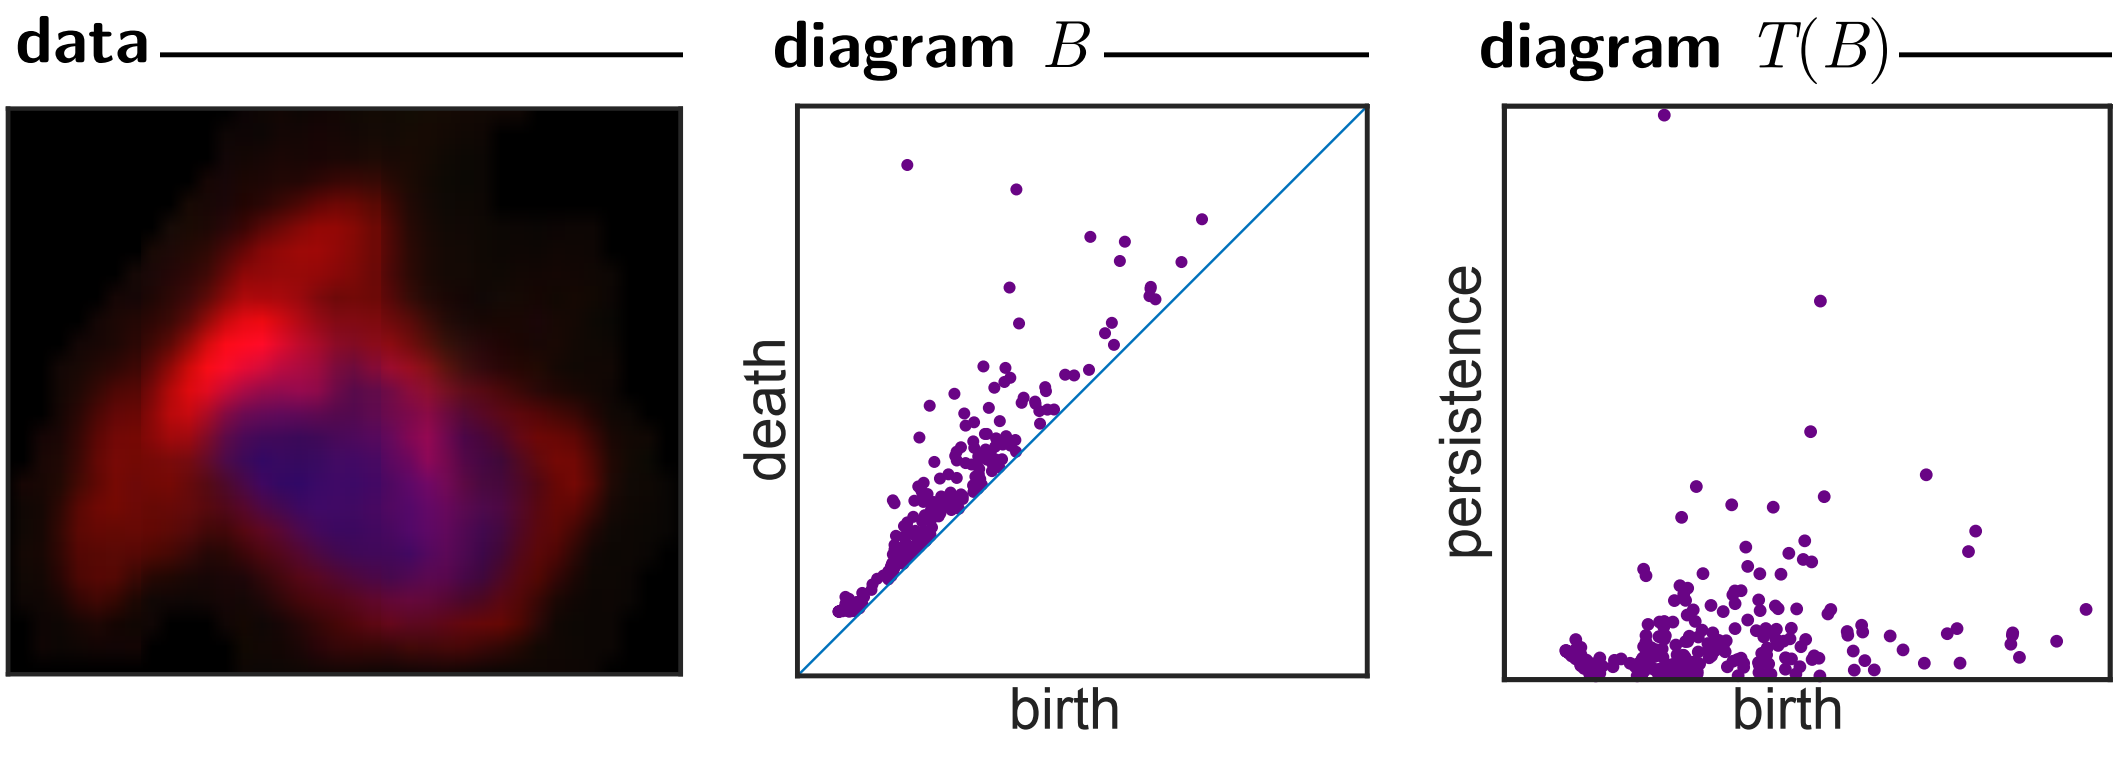
\includegraphics[width=\linewidth]{figures/persistence-images-1.png}
        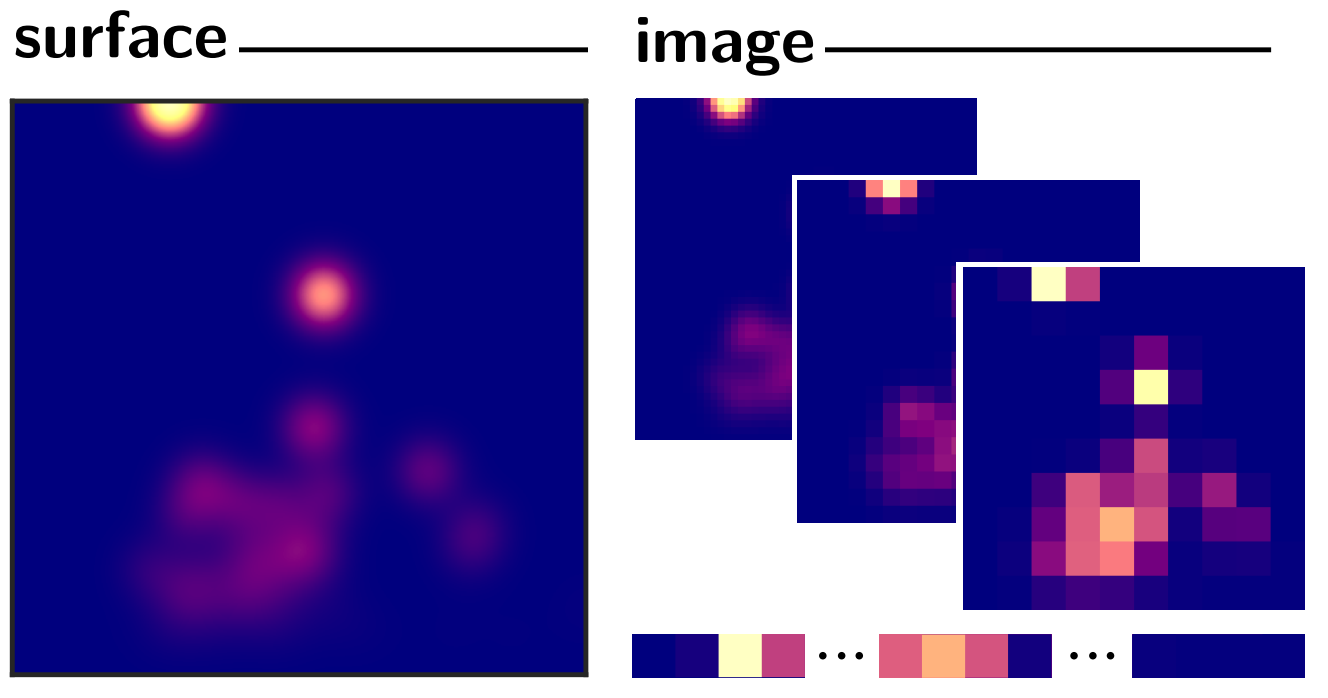
\includegraphics[width=0.66\linewidth]{figures/persistence-images-2.png}
        \caption[Persistence images pipeline]{(From \cite{adams}[Figure 1]) Algorithm pipeline to transform data into a persistence image.}
        \label{fig:persistent-images}
    \end{figure}
\end{example}

\begin{lemma}[Lemma 3, \cite{adams}] \label{lemma:images-aux}
    Let $ u, v \in \R^2 $. Fix a nonnegative weighting function $ f \colon \R^2 \to R $ that is zero along the horizontal axis, continuous and picewise differentiable. Fix a differentiable probability distribution $ \phi_u \colon \R^2 \to \R $, with mean $ u \in \R^2 $. The following inequality asserts.
    \begin{equation}
        \|f(u) \phi_u - f(v)\phi_v \|_\infty \leq (\|f\|_\infty |\nabla \phi| + \|\phi\|_\infty |\nabla f |) \| u - v \|_2.
    \end{equation}
\end{lemma}
\begin{proof}
    For any $ z \in \R^2 $ we have
    \begin{equation}
        | \phi_u(z) - \phi_v(z) | = | \phi_u(z) - \phi_u(z + u - v) | \leq |\nabla \phi | \|u - v \|_2.
    \end{equation}
    Hence,
    \begin{equation}
        \| \phi_u - \phi_v \| \leq |\nabla \phi | \|u - v \|_2.
    \end{equation}
    Applying this, we can now develop    
    \begin{align}
        |f(u)\phi_u(z) - f(v)\phi_v(z)| &= |f(u)(\phi_u(z) - \phi_v(z)) + (f(u) - f(v))\phi_v(z)| \\
        &\leq \|f\|_\infty |\phi_u(z) - \phi_v(z)| + \|\phi\|_\infty |f(u) - f(v)| \\
        &\leq \|f\|_\infty \|\nabla \phi\| \|u - v\|_2 + \|\phi\|_\infty \|\nabla f\| \|u - v\|_2 \\
        &= (\|f\|_\infty \|\nabla \phi\| + \|\phi\|_\infty \|\nabla f\|)\|u - v\|_2.
    \end{align}
\end{proof}

Persistence surfaces are stable with respect to the $1$-Wasserstein distance (see \ref{def:Wasserstein}).

\begin{theorem}[Theorem 4, \cite{adams}] \label{theorem:images-1}
    Let $ D, D' $ be two persistent diagrams and $ \rho_D, \rho_{D'} $ two  persistence surfaces associated to each diagram respectively. Then
    \begin{equation}
        \| \rho_B - \rho_{B'} \|_\infty \leq \sqrt{10} (\|f\|_\infty |\nabla \phi | + \|\phi\|_\infty |\nabla f |) \omega_1(D, D').
    \end{equation}
\end{theorem}
\begin{proof}
    Since $D$ and $D'$ consist of finitely many points, there exists a matching $\gamma$ that achieves the infimum in the Wasserstein distance. Then
    \begin{align}
        \|\rho_B - \rho_{B'}\|_{\infty} 
        &= \left\| \sum_{u \in T(B)} f(u)\phi_u - \sum_{u \in T(B)} f(\gamma(u))\phi_{\gamma(u)} \right\|_{\infty} \\
        &\leq \sum_{u \in T(B)} \left\| f(u)\phi_u - f(\gamma(u))\phi_{\gamma(u)} \right\|_{\infty},
    \end{align}
    We now apply Lemma \ref{lemma:images-aux} and then note that $ \|\cdot \|_2 \leq \sqrt{2} \| \cdot \| in \R^2 $. and that $ \|T(\cdot) \|_2 \leq \sqrt{5} \| \cdot \| $,
    \begin{align}
        \sum_{u \in T(B)} \left\| f(u)\phi_u - f(\gamma(u))\phi_{\gamma(u)} \right\|_{\infty}
        &\leq \sqrt{2} (\|f\|_{\infty} \|\nabla \phi\| + \|\phi\|_{\infty} \|\nabla f\|) 
        \sum_{u \in T(B)} \|u - \gamma(u)\|_{\infty} \\
        &\leq \sqrt{10} (\|f\|_{\infty} \|\nabla \phi\| + \|\phi\|_{\infty} \|\nabla f\|) 
        \sum_{u \in B} \|u - \gamma(u)\|_{\infty} \\
        &= \sqrt{10} (\|f\|_{\infty} \|\nabla \phi\| + \|\phi\|_{\infty} \|\nabla f\|) W_1(B, B').
    \end{align}
\end{proof}

Persistence images are stable with respect to the $1$-Wasserstein distance.

\begin{theorem}[Theorem 5, \cite{adams}] \
    Let $ A $ be be the maximum area of any pixel in the image, $ A' $ the total area of the image, and $ n $ the number of pixels in the image. Then
    \begin{align}
        &\| I(\rho_B) - I(\rho_{B'}) \|_\infty \leq \sqrt{10} A (\|f\|_\infty |\nabla \phi | + \|\phi\|_\infty |\nabla f |) \omega_1(D, D'), \\
        &\| I(\rho_B) - I(\rho_{B'}) \|_1 \leq \sqrt{10} A' (\|f\|_\infty |\nabla \phi | + \|\phi\|_\infty |\nabla f |) \omega_1(D, D'), \\
        &\| I(\rho_B) - I(\rho_{B'}) \|_2 \leq \sqrt{10n} A (\|f\|_\infty |\nabla \phi | + \|\phi\|_\infty |\nabla f |) \omega_1(D, D'). \\
    \end{align}
\end{theorem}
\begin{proof}
    Note for any pixel $ p $ with area $ A(p) $ we have
    \begin{align}
        |I(\rho_{B})_{p} - I(\rho_{B'})_{p}| &= \left| \iint_{p} \rho_{B} \, dy dz - \iint_{p} \rho_{B'} \, dy dx \right| \\
        &= \left| \iint_{p} \rho_{B} - \rho_{B'} \, dy dx \right| \\
        &\leq A(p) \|\rho_{B} - \rho_{B'}\|_{\infty} \\
        &\leq \sqrt{10} A(p) \big( \|f\|_{\infty} |\nabla \phi| + \|\phi\|_{\infty} |\nabla f| \big) \omega_{1}(B, B'),
    \end{align}
    where the last inequality comes by applying Theorem \ref{theorem:images-1}. Hence we have
    \begin{align}
        \|I(\rho_{B}) - I(\rho_{B^{\prime}})\|_{\infty} &\leq \sqrt{10}A(\|f\|_{\infty}|\nabla\phi| + \|\phi\|_{\infty}|\nabla f|\big)\omega_{1}(B,B^{\prime}) \\
        \|I(\rho_{B}) - I(\rho_{B^{\prime}})\|_{1} &\leq \sqrt{10}A^{\prime}\big(\|f\|_{\infty}|\nabla\phi| + \|\phi\|_{\infty}|\nabla f|\big)\omega_{1}(B,B^{\prime}) \\
        \|I(\rho_{B}) - I(\rho_{B^{\prime}})\|_{2} &\leq \sqrt{n}\|I(\rho_{B}) - I(\rho_{B^{\prime}})\|_{\infty} \\
        &\leq \sqrt{10n}A\big(\|f\|_{\infty}|\nabla\phi| + \|\phi\|_{\infty}|\nabla f|\big)\omega_{1}(B,B^{\prime}).
    \end{align}
\end{proof}

\section{Euler curves}  \label{sec:euler-curves}

The Euler characteristic curve provides a concise topological signature by tracking the evolution of the Euler characteristic across a filtration. This section examines its definition, connection to persistence diagrams, and stability properties, demonstrating how it serves as a stable summary for comparing filtered cell complexes.

\begin{definition}[Euler characteristic]
    Let $ K $ be a simplicial complex, and let $ K^p $ be its $p$-skeleton. The {\bf Euler characteristic} of $ K $ is the alternating sum of the number of cells in its dimension
    \begin{equation}
        \chi(K) \coloneq \sum_d (-1)^d \#(K^d).
    \end{equation}
\end{definition}

\begin{definition}
    Let $ K $ be a simplicial complex. Let $ f \colon K \to \R $ be a filtration function. The {\bf Euler characteristic curve} is a function that assign an Euler characteristic $ \chi $ for each filtration level $ t \in \R $. 
    \begin{equation}
        \ecc(K, t) \coloneq \chi(K_t),
    \end{equation}
    where $ K_t = f^{-1} (-\infty, t] $.
\end{definition}

Using the $L_1$ norm, we can measure distances between Euler curves of different filtered simplicial complexes in a manner that results to be stable.

\begin{definition}[$k$-th Betti curve]
    Let $ K $ be a simplicial complex with filtration function $ f \colon K \to \R $. Its {\bf $k$-th Betti curve} is a function that assigns a Betti number for each filtration level $t \in \R $.
    \begin{equation}
        \beta_k(K, t) \coloneq \beta_k(K_t).
    \end{equation}
\end{definition}

\begin{definition}[\bf $k$-th Betti curve for a persistence diagram]
    Let $ D $ be a persistence diagram. Given a point $ (b,d) \in D $, let $ I_{[b,d)} $ be the indicator function defined as
    \begin{equation}
        I_{[b,d)}(t) \coloneq \begin{cases}
            1 &\text{ if } t \in [b,d), \\
            0 &\text{ otherwise}.
        \end{cases}
    \end{equation}
    The {\bf $k$-th Betti curve for a persistence diagram $ D $} with finitely many off-diagonal points is defined as
    \begin{equation}
        \beta_k(D, t) = \sum_{(b, d) \in D} I_{[b,d)}(t).
    \end{equation}
\end{definition}

\begin{proposition}[Proposition 1, \cite{dlotko}] \label{prop:curves}
    Let $ D $, $ D' $ be two $ k$-dimensional persistence diagrams. Their Betti curves are stable respect the 1-Wasserstein distance,
    \begin{equation}
        \| \beta_k(D, t) - \beta_k(D', t) \|_1 \leq 2 \omega_1(D, D').
    \end{equation}
\end{proposition}
\begin{proof}
    Order the points in each diagram $ (b_i, d_i) \in D $, and  $ (b_i', d_i') \in D' $ such that points with the same index $ i $ are paired by the optimal matching given by the 1-Wasserstein distance. We then can write the difference between the two Betti curves as
    \begin{equation}
        \|\beta_k(D, t) - \beta_k(D', t)\|_1 = \| \sum_i \left(I_{[b_i, d_i)}(t) - I_{[b_i', d_i')}(t)\right)  \|_1 
        \leq \sum_i \| \left(I_{[b_i, d_i)}(t) - I_{[b_i', d_i')}(t)\right)  \|_1.
    \end{equation}
    We can now focus on each term of the sum and differentiate three cases. Case 1 comes up when $ b_i \leq b_i' \leq d_i \leq d_i' $. Unfolding $ L_1 $ norm we get 
    \begin{align}
        \|  \! \left(I_{[b_i, d_i)}(t) - I_{[b_i', d_i')}(t)\right) \! \|_1 &=
        \! \! \int_{b_i}^{b_i'} \left| I_{[b_i, d_i)(t)}\right| dt + \! \! \int_{b_i'}^{d_i} \left| I_{[b_i, d_i)(t)} - I_{[b_i', d_i')(t)}\right| dt + \! \! \int_{d_i}^{d_i'} \left| I_{[b_i', d_i')(t)}\right| dt \\
        &= \int_{b_i}^{b_i'} \left| 1 \right| dt + \int_{b_i'}^{d_i} \left| 1-1 \right| dt + \int_{d_i}^{d_i'} \left|1\right| dt \\
        &= |b_i' - b_i| + |d_i' - d_i| \leq 2 \max(|b_i' - b_i|, |d_i' - d_i|).
    \end{align}
    Case 2 comes up when $ b_i \leq b_i' \leq d_i' \leq d_i $, getting
    \begin{align}
        \|  \! \left(I_{[b_i, d_i)}(t) - I_{[b_i', d_i')}(t)\right) \! \|_1 &=
        \int_{b_i}^{b_i'} \left| 1 \right| dt + \int_{b_i'}^{d_i'} \left| 1-1 \right| dt + \int_{d_i'}^{d_i} \left|1\right| dt \\
        &= |b_i' - b_i| + |d_i - d_i'| \leq 2 \max(|b_i' - b_i|, |d_i' - d_i|).
    \end{align}
    A degenerate case 2 comes when some point $ (b_i, d_i) \in C $ is matched to a point in the diagonal of $ D $, and thus $ b_i \leq b_i' = d_i' \leq d_i $. The final posible case comes when $ b_i \leq d_i \leq b_i' \leq d_i' $, but this will never happen as if so, a better matching between the diagrams can be found matching both points to the diagonal.

    Summing up both posible cases we complete the proof as
    \begin{align}
        \|\beta_k(D, t) - \beta_k(D', t)\|_1 &  = \| \sum_i \left(I_{[b_i, d_i)}(t) - I_{[b_i', d_i')}(t)\right)  \|_1 \\
        &\leq \sum_i 2 \max(|b_i' - b_i|, |d_i' - d_i|) = 2 \omega_1 (D, D').
    \end{align}
\end{proof}

\begin{theorem}[Proposition 2, \cite{dlotko}]
    Let $ X, Y $ be two filtered cell complexes and let $ D(X), D(Y) $ be its respective persistence diagrams. Then,
    \begin{equation}
        \| \ecc(X, t) - \ecc(Y, t) \|_1 \leq \sum_k 2 \omega_1(D(X), D(Y)).
    \end{equation}
\end{theorem}
\begin{proof}
    The Euler-Poincaré formula implies that we can express the Euler characteristic curve of a filtered simplicial complex $K $ as the alternating sum of its Betti curves. That is
    \begin{align}
        \ecc(K, t) = \sum_k(-1)^k \beta_k(K, t).
    \end{align}
    Hence, applying Proposition \ref{prop:curves} and the triangular inequality we get
    \begin{align}
        \| \ecc(X, t) - \ecc(Y, t) \|_1 &= \| \sum_{k=0}^n \left( (-1)^k (\beta_k(D(X), t) - \beta_k(D(Y), t)) \right)\|_1 \\
        &\leq \sum_{k=0}^n \|(\beta_k(D(X), t) - \beta_k(D(Y), t))\|_1 \\
        &\leq \sum_{k=0}^n 2 \omega_1(D(X), D(Y)).    
    \end{align}
\end{proof}
